\documentclass[11pt]{article}
\usepackage[margin=1in]{geometry}
\usepackage{graphicx}
\usepackage{microtype}
\usepackage{verbatim}
\usepackage{amsmath}
\usepackage{nicefrac}
\usepackage[colorlinks=false, hidelinks]{hyperref}
\usepackage{caption}
\usepackage{subcaption}
\usepackage{listings}
\usepackage{harmony}
\usepackage{wasysym}

\begin{document}

\title{LFSR and ASG Pseudorandom Number Generators\\Embedded System Design, Lab 5}
\date{October 22, 2015}
\author{Ben Lorenzetti}
\maketitle

\tableofcontents

\clearpage

\section{Objectives and Problem Descriptions}
\subsection{8-Bit Linear Feedback Shift Register (LFSR)}
\label{problem-1-specs}

Implement an 8--bit linear feedback shift register (LFSR) on the PIC16F877 44--Pin Demo Board.
The LFSR should be designed with suitable taps such that 255 unique numbers are produced in a
pseudorandom sequence before the cycle repeats.

The 8--bits should be displayed on the 8 LEDs connected to Port D on the demo board.
The LFSR should cycle (change state) once per second.

\subsection{Alternating Step Generator (ASG)}
\label{problem-2-spces}

Implement an alternating step generator (ASG) on the PIC16F877 44--pin demo board.
The ASG should be comprised of three LFSRs with 14--bit, 15--bit, and 16--bit
lengths. The pseudorandom bit sequence produced by the ASG should be displayed
on the 8 LEDs on board the 44--pin demo board. Eight new bits should be displayed
every second.

The ASG should be implemented with suitable taps such that each LFSR produces the
maximum length sequence for it's bit size. One LFSR should be cycled each iteration,
and the output bit from this LFSR should be used to select one of the other two.
From the other two LFSRs, the register which is cycled produces the output bit
of the ASG for that cycle.

\section{Procedure}
\subsection{Reading Assignments}

The lab procedure and the blackboard post had a cornucopia of reading assignments,
including the user manuals for MPLAB X IDE, the PIC Assembler, the 44--pin demo board,
and online getting started guides.

There was way to much to actually read, but some of it was helpful. Particularly
the first sections of the online getting started with MPLAB guide and the Assembler
Users Manual. The PIC16F877 datasheet was also useful since the PDF is searchable.

\subsection{LFSRs and ASGs Theory}

A linear--feedback shift register (LFSR) is a shift register whose input is a linear,
real time function of its current state.

Usually the linear function is a cascade of XOR gates that ``tap'' some of the upper
order bits on the LFSR. The tapped bits are know as the feedback polynomial for the
LFSR. If the feedback function is constructed as a cascade of XOR gates, the LFSR
is known as a Fibonacci LFSR. An example of a 14--bit Fibonacci LFSR is shown 
in figure \ref{14-bit-fibonacci-with-feedback-polynomial}.

\begin{center}
	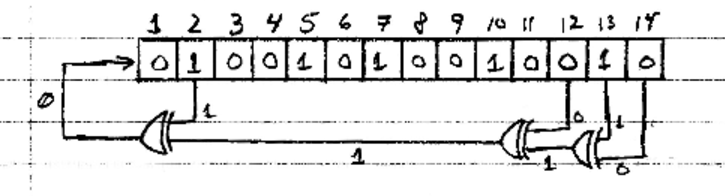
\includegraphics[width=0.7\textwidth]{Figures/14-bit-fibonacci-with-feedback-polynomial.pdf}
	\captionof{figure}{A 14-bit Fibonacci LFSR with feedback polynomial $F(x)=x^{14}+x^{13}+x^{12}+x^{2}+1$}
	\label{14-bit-fibonacci-with-feedback-polynomial}
\end{center}

LFSRs are often used as pseudorandom number generators and the initial value is know
as the ``seed'' value. For Fibonacci LFSRs, a seed value of zero will cause the LFSR
to be forever stuck in the zero state.

If the feedback polynomial is chosen correctly, the LFSR can produce $2^{n}-1$
(not including 0) pseudorandom numbers before the sequence begins to repeat.
It turns out that all of the LFSRs of bit length $n$ with a sequence $2^{n}-1$
long have some similarities. They have an even number of taps and all of the tap
locations, taken together, must be relatively prime. For example, an LFSR tapped
at bits 2 and 4 or 2 and 8 would certainly not have the maximum sequence length.
Some feedback polynomials that are know to produce maximum length sequences are
listed in table \ref{feedback-polynomials-table}.

\begin{table}
\centering
\caption{Feedback Polynomials with Maximum Length Sequences}
\begin{tabular}{c | l | c | c}
\hline\hline
Size of LFSR	&Feedback Polynomial	&Sequence Length	&\texttt{TAP\_MASK}	\\
\hline
3--bits	&$x^{3}+x^{2}+1$		&7	&\texttt{0x0006}	\\
4--bits	&$x^{4}+x^{3}+1$		&15	&\texttt{0x000C}	\\
5--bits	&$x^{5}+x^{3}+1$		&31	&\texttt{0x0014}	\\
6--bits	&$x^{6}+x^{5}+1$		&63	&\texttt{0x0030}	\\
7--bits	&$x^{7}+x^{6}+1$		&127	&\texttt{0x0060}	\\
8--bits	&$x^{8}+x^{6}+x^{5}+x^{4}+1$	&255	&\texttt{0x00D8}	\\
14--bits&$x^{14}+x^{13}+x^{12}+x^{2}+1$	&16383	&\texttt{0x3802}	\\
15--bits&$x^{15}+x^{14}+1$		&32767	&\texttt{0x6000}	\\
16--bits&$x^{16}+x^{14}+x^{13}+x^{11}+1$&65535	&\texttt{0xB400}	\\
\hline\hline
\end{tabular}
\label{feedback-polynomials-table}
\end{table}

\subsection{Implementation Design}

\begin{figure}
	\centering
	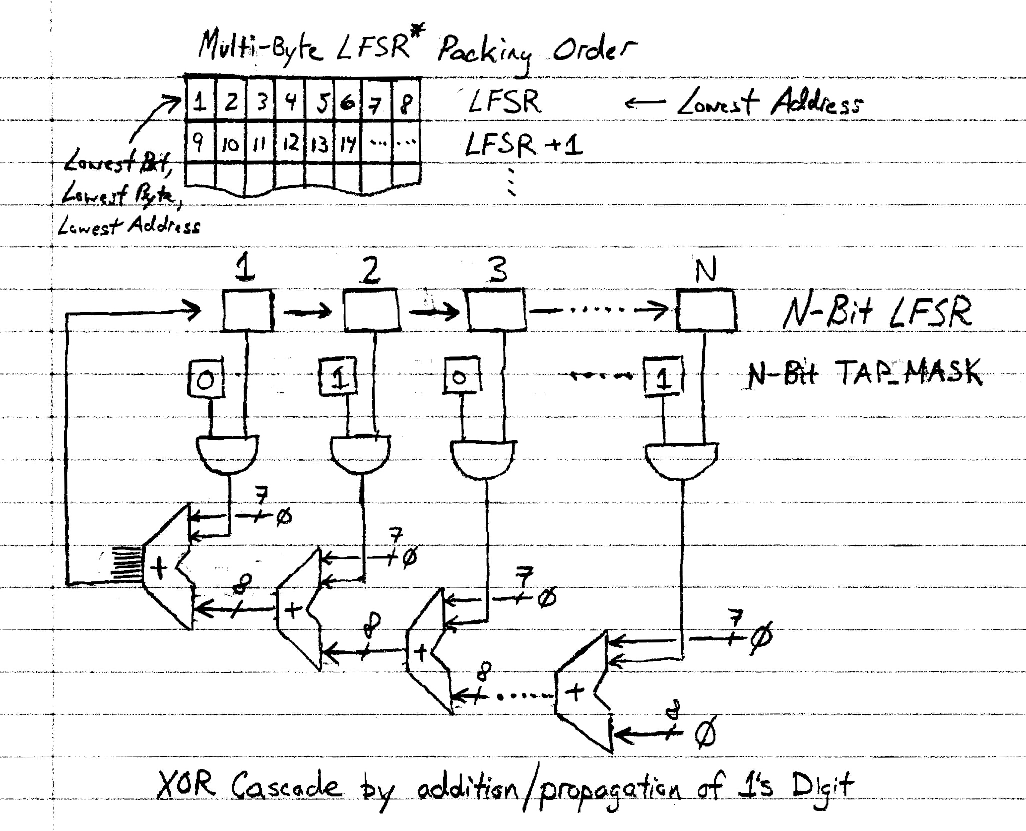
\includegraphics[width=0.75\textwidth]{Figures/fibonacci-equivalent-circuit.pdf}
	\caption{Equivalent Circuit Implementation of an Arbitrary Length Fibonacci LFSR}
	\label{fibonacci-equivalent-circuit}
\end{figure}

Bitwise manipulation is always difficult in any programming language because
computers and microcontrollers are designed to use data in groups of bytes---or
whatever the word size of the machine may be.

Luckily, the PIC instruction set has rotate left and rotate right instructions
which can shift bits in and out of a byte like a queue. Nine bits are involved,
eight bits from the byte being rotated and a ninth bit---the carry flag from
the status register. The \texttt{STATUS, C} flag is set by many ALU operations but, in the case
of rotate left and rotart right, the value in the Carry Flag is shifted into
the byte and is replaced by the value shifting out the other side of the byte queue.
The assembler mnemonics for rotate left and rotate right are:
\begin{verbatim}
  RLF  f, d  ; f is address of the operand value and d is result destination
  RRF  f, d  ; d=1 stores result back at ADDR f, d=0 stores result in W
\end{verbatim}

My design for a generic length LFSR takes takes advantage of these rotate instructions.
The hardware concept for my design is shown in figure \ref{fibonacci-equivalent-circuit}.
This arrangement of hardware lends itself to implementable in software because there are few
conditional statements; the XOR cascade can be implemented as a loop instead of
a unique--per--feedback--polynomial sequence of logic statements. Also, instead of
trying to arrange bits to overlap for \texttt{XOR} operations, it propagates the
XOR signal in the 1's Digit of a register with repeated addition of \texttt{0} or \texttt{1}.
This has an effect equivalent to XORing if you ignore the higher order bits.

\begin{figure}
	\centering
	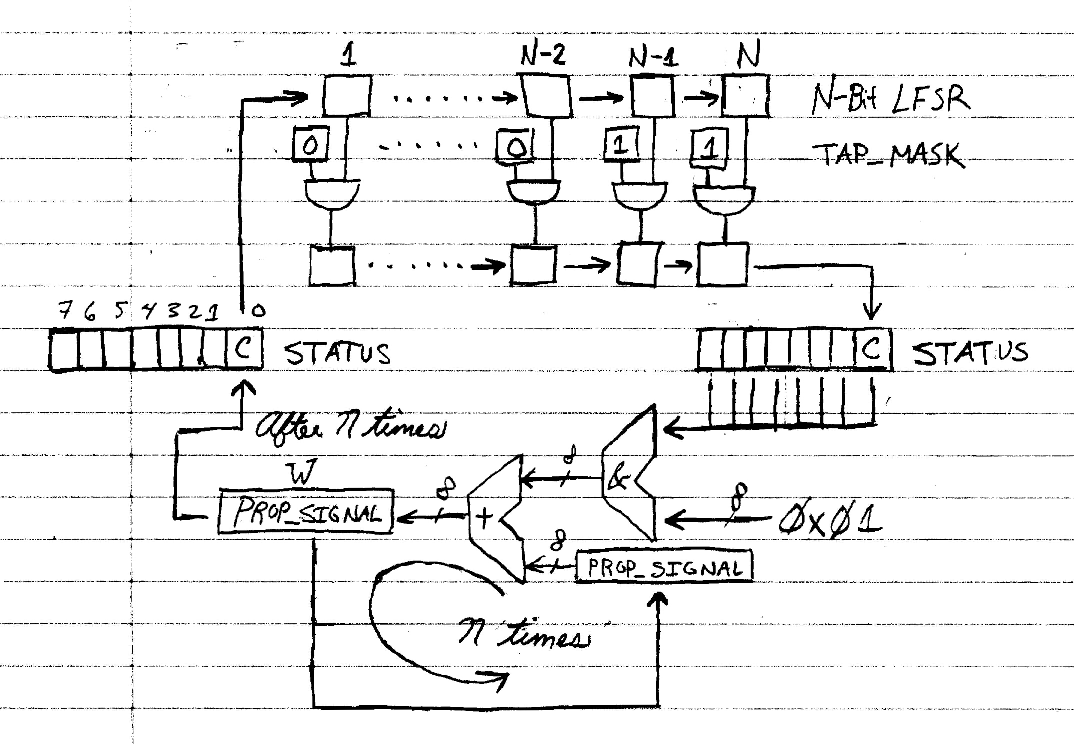
\includegraphics[width=0.75\textwidth]{Figures/xor-propagation-flowchart.pdf}
	\caption{Implementation of XOR Propagation}
	\label{xor-propagation-flowchart}
\end{figure}

Since LFSRs are easily visuallized as hardware, a flowchart for the XOR function
implementation is similarly drawn in figure \ref{xor-propagation-flowchart}.
This flowchart shows the value of the PIC architecture's Carry Flag for implementing an LFSR.

\begin{figure}
	\centering
	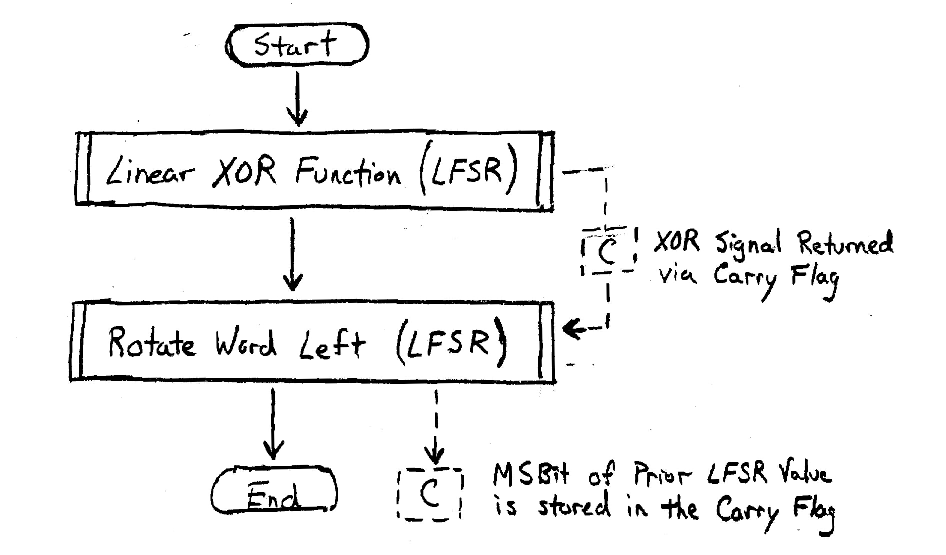
\includegraphics[width=0.6\textwidth]{Figures/cycle-lfsr-flowchart.pdf}
	\caption{Cycle LFSR Function Implementation Flowchart}
	\label{cycle-lfsr-flowchart}
\end{figure}

The full process of advancing to the next state in the LFSR sequence involves
calculating the result of the linear XOR function and then shifting the LFS register
by 1--bit with the XOR result as input. This is shown in the implementation
flowchart in figure \ref{cycle-lfsr-flowchart}.

\subsection{Hello World Program (Delay Function)}

One of the requirements for both the 8--bit LFSR and the ASG is that
the LED display should change at a rate of 1 Hz. The PIC16F887 on
the demo board executes instructions at 1 MHz, so there will obviously
need to be a delay after the microcontroller has calculated the next
value, but before it should be displayed.

Since I have never programmed a PIC controller and since most 
microcontroller \texttt{hello\_world} programs are blinking LEDs with
a time delay, this was a logical first function to implement.

In the listing in \hyperref[lfsr-code]{section \ref{lfsr-code}},
the delay function is labeled \texttt{Pause\_1\_Second} and
consists of three nested loops and a fourth fudge factor loop.
In theory these loops could be tuned based on the number of instructions
in the final, debugged program to produce an exact 1 Hz cycle.
I am far to lazy to do this though.

I am predjudiced against integrated development environments because
they obscure what is happening between your code text and the machine.
I think they make programmers subconsciously bounded within a box.
If you are going to learn a complicated piece of software, just learn
the operating system---not a random IDE.

This is also why I avoid MATLAB. Perhaps an exception would be LISP if
I ever bothered to learn it, because the IDE could be, inceptionally, LISP itself.

Anyway, my \texttt{.asm} source files were assembled on the command line so
please do this if they don't compile nicely in the IDE.
On Ubuntu, with the default MPLAB installation location, 
from the directory containting \texttt{lfsr.asm}, the commands are:
\begin{verbatim}
$ cp /opt/microchip/mplabx/v3.10/mpasmx/p16f877.inc ./p16f887.inc
$ /opt/microchip/mplabx/v3.10/mpasmx/mpasmx -p16f887 lfsr.asm
$ more lfsr.ERR
\end{verbatim}

\subsection{Assembly Macros (Rotate Word Function)}

The \texttt{RRF} and \texttt{RLF} instructions only operate on a single
byte of data. Looking at my implementation design
(\hyperref[fibonacci-equivalent-circuit]{figure \ref{fibonacci-equivalent-circuit}} and
\hyperref[xor-propagation-flowchart]{figure \ref{xor-propagation-flowchart}}),
a function that is needed often is rotating word variables of multiple bytes.

The function needs to work for different word variable addresses and different byte lengths.
It should also function just like \texttt{RRF} and \texttt{RLF} in terms of the
\texttt{STATUS, C} flag.

I implemented this function with an assembly macro labeled \texttt{RLF\_Word}
in \hyperref[lfsr-code]{section \ref{lfsr-code}} and \ref{asg-code}.

\subsection{XOR Propagation Function}

The linear exclusive or cascade also lends itself to a macro, because
it requires making a ``function scope'' copy of the \texttt{LFSR} variable
ANDed with a \texttt{TAP\_MASK}. These variables are potentially words of
multiple byte length, and the programmer should not have to manually add
and remove lines based on the number of bytes desired. This can be automated
by the assembler.

My design for the LFSR concentrates all of the bit--packing operations
for multiple--byte LFSRs into the Rotate\_Word function, so the XOR code
does not need to have outer loops and indirect addressing nonsense for
accessing the correct byte; the bit needed for every iteration is preplaced
in the carry flag.

The XOR function is implemented in both code implentations at the
label \texttt{Linear\_Xor\_Function}.

\subsection{8-Bit LFSR Design}

\begin{figure}
	\centering
	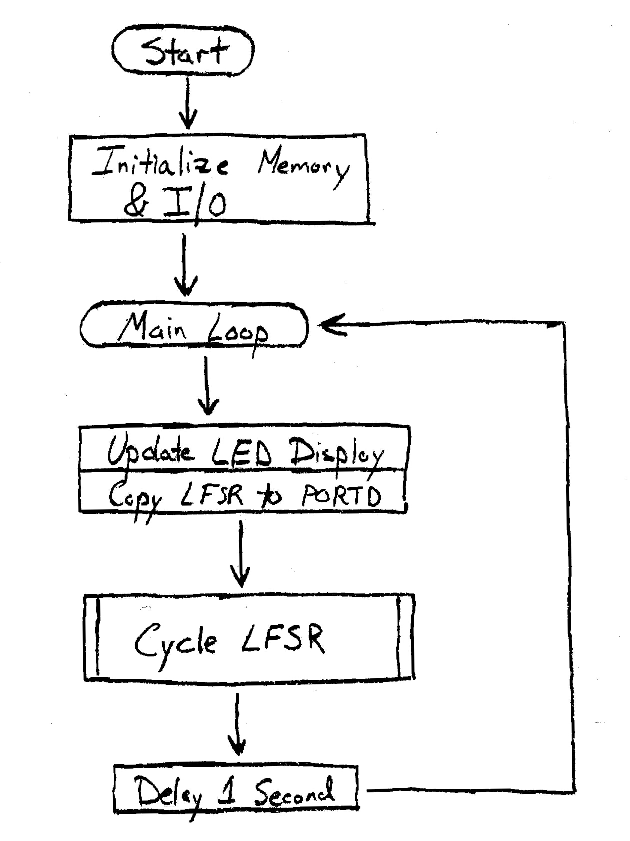
\includegraphics[width=0.35\textwidth]{Figures/8-bit-lfsr-flowchart.pdf}
	\caption{8-Bit LFSR Implementation Flowchart}
	\label{8-bit-lfsr-flowchart}
\end{figure}

For the first objective of the lab, my implementation is outlined in the
flowchart in \hyperref[8-bit-lfsr-flowchart]{figure \ref{8-bit-lfsr-flowchart}}.
The assembly source code is listed in
\hyperref[lfsr-code]{section \ref{lfsr-code}}.

Almost everything needed for the implementation is handled by the two subroutines
discussed above, \texttt{RLF\_Word} and \texttt{Linear\_Xor\_Function}.

The LFSR bit size and feedback polynomial can be changed easily by the programmer.
Simply re\texttt{\#define} the literal values for \texttt{LFSR\_SIZE} and
\texttt{LFSR\_TAP\_MASK}. Tap masks for several bit size LFS registers are listed
in \hyperref[feedback-polynomials-table]{table \ref{feedback-polynomials-table}}.

\pagebreak
\subsection{ASG Design}

My implementation for the alternating step generator is shown in
\hyperref[alternating-step-generator-flowchart]{figure \ref{alternating-step-generator-flowchart}}.
The assebly source code is listed in \hyperref[asg-code]{section \ref{asg-code}}.

Again, almost everything needed for the implementation is handled by the two
MACROs \texttt{RLF\_Word} and \texttt{Linear\_Xor\_Function}.

For each of the 3 feedback shift registers, the bit sizes and tap locations
are defined by assembler literals in lines 11--18.

\begin{figure}
	\centering
	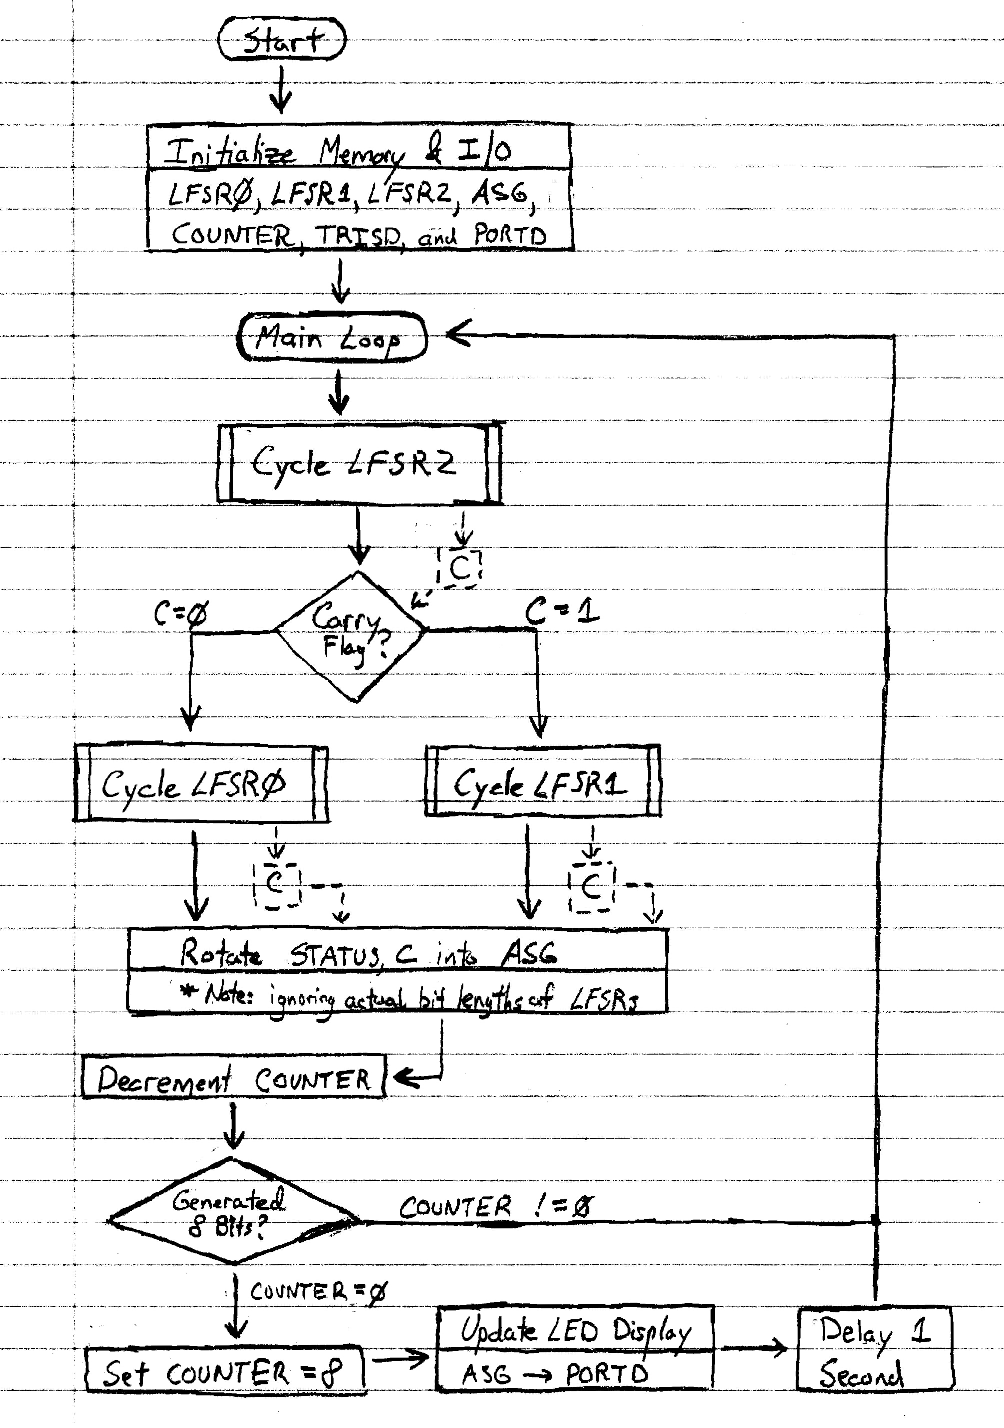
\includegraphics[width=0.6\textwidth]{Figures/alternating-step-generator-flowchart.pdf}
	\caption{Alternating Step Generator Implementation}
	\label{alternating-step-generator-flowchart}
\end{figure}

\pagebreak
\section{Expected Results}

\subsection{3-Bit LFSR Demonstration}

To demonstrate that my implementations of the feedback shift registers
is functioning correctly, I edited the \texttt{LED\_MASK} and
\texttt{LFSR1\_TAP\_MASK} to produce a 3--bit LFSR.
\begin{verbatim}
#define  LED_MASK        0x07   ; mask all but low 3 LEDs
#define  LFSR1_TAP_MASK  0x06   ; tap bits 2 and 3 (2 + 4 = 6)
\end{verbatim}

For 3--bits,
one can manually observe the sequence of random numbers because
the period is only 7 numbers long.

\subsection{8-Bit LFSR Demonstration}

For this demonstration, I expected the LEDs to cycle through 255 unique
numbers at approximately 1 Hz.

\subsection{ASG Demonstration}

For this demonstration, I expected sequence of numbers that appears
random. The length of the sequence before it begins to repeat is far
to large to test experimentally.

\section{Experiment and Design Revisions}

\subsection{Addition of Macros}

In my original implementations, I did not write macros for rotating multi--byte
words or for making local copies of the LFSR words for the XOR propagation function.
I had intentially designed both of these functions to scale easily to the 2--byte,
3--LFSR needs of ASG, and MACROs turned out to be the way to program it easily in assembly.

\subsection{Use of Carry Flag between Functional Blocks}

When I first implemented the two macro functions, I did not use the carry
bit for the return value because I was worried about accidentally doing
another ALU operation in between the macro return and the use of the result.

Upon closer examination, I was able to reorganize the instructions both
inside and outside the macros so that the carry bits always remained valid and
could be used for the function returns.

It was very convenient that the folks at PIC did not make the decrement instructions
affect \texttt{STATUS, C}.

\section{Observations}

\subsection{Observations}

\begin{center}
	\includegraphics[width=0.5\textwidth]{Figures/3-bit-lfsr-demo.jpg}
	\captionof{figure}{Demonstration of 3--Bit LFSR}
	\label{3-bit-lfsr-demo-jpg}
\end{center}

\section{Discussion}

I think I already discussed a lot about PIC assembly in earlier sections.

I am very impressed by the value created by the folks at PIC when
they placed the carry flag in the $0^{\textrm{th}}$ bit of the status
register and by the side effect functionallity of this bit with arithmetic
instructions. Having the carry bit in the 1's digit allowed me to do
my XOR propagation without having to do any bit manipulations.
I am also appreciative of their choice not to have decrement operations
affect the carry flag. This is very convenient because loop iterations
do not invalidate the carry flag.

This was my first time programming in assembly and using the MPLAB
integrated development environment. Unfortunately I spend a lot of
frustrating time searching for settings and inexplicable debugging
when trying to use the IDE. In the end I gave up and reverted to my
comfort zone, compiling on the command line. If I get fancy I might
write a makefile script. I think this is either a flaw about myself
or about IDEs in general, not necessarily about MPLAB.

\clearpage
\section{Implementation Code}

\subsection{8-Bit LFSR}
\label{lfsr-code}

\lstinputlisting[breaklines, basicstyle=\small]{Eight-Bit-LFSR/lfsr.asm}


\clearpage
\subsection{Alternating Step Generator}
\label{asg-code}

\lstinputlisting[breaklines, basicstyle=\small]{Alternating-Step-Generator/asg.asm}



\end{document}
